\section{Implementation}
\begin{frame}
    \sectionpage
\end{frame}

\begin{frame}{Starting point}
    HQC has two software implementations
    \begin{block}{HQC implementations}
        \begin{itemize}
            \item \texttt{reference}: implemented in C, no optimizations, not constant-time, sparse-dense multiplications
            \item \texttt{optimized}: implemented using AVX2 instructions, vectorized decoding, Karatsuba dense-dense multiplications
        \end{itemize}
        Our implementation starts from the \texttt{reference}.
    \end{block}
\end{frame}

\begin{frame}{Target architecture}
    Our implementation is oriented torwards embedded devices
    \begin{columns}
        \begin{column}{0.45\linewidth}
            \begin{block}{Target}
                Our target is the STM32F401RE board:
                \begin{itemize}
                    \item Cortex-M4 processor (\texttt{ARMv7E} architecture)
                    \item 512KB Flash Memory
                    \item 96KB RAM
                    \item No builtin RNG
                \end{itemize}
            \end{block}
        \end{column}
        \begin{column}{0.45\linewidth}
            \begin{figure}
                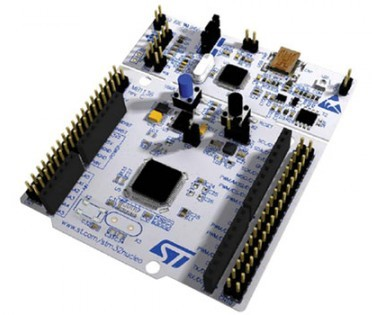
\includegraphics[scale=0.5]{images/stm32board.jpg}
            \end{figure}
        \end{column}
    \end{columns}   
\end{frame}


\begin{frame}{Objects representations}
    \begin{block}{}
        \begin{itemize}
            \item Random values: generated from a 40B seed with \texttt{seedexpander} functions
            \item Codewords: as polynomials (through arrays), in two possible forms:
            \begin{itemize}
                \item dense: each bit represents a coefficient of the corresponding degree, implemented with \texttt{uint64\_t} arrays of \texttt{VEC\_N\_SIZE\_64} elements
                \item sparse: elements correspond to the degrees with nonzero coefficient, implemented with \texttt{uint32\_t} arrays of \texttt{PARAM\_OMEGA} elements
            \end{itemize}
        \end{itemize}
    \end{block}
\end{frame}

\begin{frame}{Masking}
    \begin{block}{Shares representations}
        The number of shares is a parameter of the cryptosystem, defined at compile time.\\
        Shares are defined via the \texttt{shares\_t} struct, containing a number of dense vectors equal to the number of shares
    \end{block}
    \begin{block}{Splitting secrets into shares}
        The arrays containing secret data are divided in a number of blocks equal to the number of shares.\\
        Each block is copied in the corresponding share, and elements outside the block are zeroed.
    \end{block}
\end{frame}

\begin{frame}{Operations on shares}
    \begin{block}{Reducing shares to an array}
        When operations on secret data are completed, the shares of the secret element are added together with a XOR.
    \end{block}
    \begin{block}{Adding shares}
        When adding up two \texttt{shares\_t} a random mask is generated and \textit{distributed} among the shares, so that by reducing to a single element
        the random mask cancels out.
    \end{block}
\end{frame}

\begin{frame}{Multiplication}
    \begin{block}{}
        In the optimized version the authors employ a Karatsuba dense-dense multiplication strategy
        \begin{itemize}
            \item Makes the operation time-constant (with some tweaks)
            \item Is significantly slower than the sparse-dense strategy
        \end{itemize}
        The sparsity of the operands (17669 vs 75) makes the preexisting sparse-dense multiplication more suitable in our case.
    \end{block}
    \begin{block}{Sparse-dense multiplication}
        Variation of the schoolbook shift-and-add strategy.\\
        Let $A$ be the dense polynomial, $B$ the sparse one, we have $A\cdot X^{B_i} = A\cdot X^{B_i \mod ts} \cdot X^{\lfloor \frac{B_i}{ts}\rfloor}$
    \end{block}
\end{frame}

\begin{frame}{Multiplication masking}
    \begin{block}{\texttt{safe\_mul}}
        Application of the Rivain-Prouff scheme:
        \begin{itemize}
            \item Operand size is reduced
            \item Apply polynomial reduction modulo $x^n+1$ to multiplication results
            \item Loop unrolling
        \end{itemize}
    \end{block}
    \begin{block}{Where to apply \texttt{safe\_mul}}
        The masked multiplication is more expensive, so it is applied only to calculate:
        \begin{itemize}
            \item Encryption: $\mathbf{s}\cdot \mathbf{r}_2$ (to calculate $\mathbf{v}$)
            \item Decryption: $\mathbf{u \cdot y}$ (to calculate the codeword to decode)
        \end{itemize}
    \end{block}
\end{frame}

